

\chapter{Block Ciphers}


\begin{definition}[Block Ciphers]\ \\
    Let $k,n$ be positive integers. A block cipher with key length $k$ and block length $n$ is an efficient keyed permutation 
    $$F: \{0,1\}^k \times \{0,1\}^n \to \{0,1\}^n$$
    
    \textbf{Remark:}
    \begin{itemize}
        \item The function $F_K := F(K,\cdot)$ is a bijection (its inverse is denoted $F_K^{-1}$).
        \item Both $F_K$ and $F_K^{-1}$ are efficiently computable given the key $K$.
        \item A secure block cipher should "behave as a pseudorandom permutation".
    \end{itemize}
\end{definition}


\section{A Note on the Concrete Security Setting}
	The key length and block length of block ciphers are fixed $\to$ no varying "security parameter". In practice:
	\begin{itemize}
	    \item actual (not asymptotic) complexity of adversaries is considered.
	    \item a block cipher is considered secure as long as no attack significantly faster than exhaustive key search exists.
	\end{itemize}


\section{Security Definition - Indistinguishability from a Random Permutation}
	\begin{definition}[$(q,t,\epsilon)$-prp secure]\ \\
	    A block cipher $F$ with key length $k$ and block length $n$ is $(q,t,\epsilon)$-prp secure if, for every probabilistic adversary $D$ 
	    that runs in time at most $t$ and deals at most $q$ oracle queries, one has
	    $$Adv_F^{prp}(D) := \vert Pr[D^{F_K(\cdot)}=1]-Pr[D^{f(\cdot)}=1] \vert \leq \epsilon,$$
	    where the first probability is taken over the uniformly random draw of $K$ and the second one over the uniformly random draw of the permutation $f: \{0,1\}^n \to \{0,1\}^n$.
	\end{definition}

	\begin{definition}[$(q,t,\epsilon)$-sprp secure]\ \\
	    A block cipher $F$ with key length $k$ and block length $n$ is $(q,t,\epsilon)$-sprp secure if, for every probabilistic adversary $D$ 
	    that runs in time at most $t$ and deals at most $q$ oracle queries, one has
	    $$Adv_F^{sprp}(D) := \vert Pr[D^{F_K(\cdot),F_K^{-1}(\cdot)}=1]-Pr[D^{f(\cdot),f^{-1}}=1] \vert \leq \epsilon,$$
	    where the first probability is taken over the uniformly random draw of $K$ and the second one over the uniformly random draw of the permutation $f: \{0,1\}^n \to \{0,1\}^n$.
	\end{definition}
	    \textbf{Remark:}\newline
	    $F$ is considered "secure" as long as $Adv_F^{sprp}(D) \leq c_1 \frac{t/T_F}{2^k} + c_2 \frac{q}{2^n}$, where $c_1$ and $c_2$ 
	    are small constants and $T_F$ is an upper bound on the time required to evaluate $F$.


\section{A word on Provable Security}
	\begin{itemize}
	    \item Typically, the security of block ciphers is not provable.
	    \item The pseudorandomness of a block cipher is actually used as an assumption in security proofs for block cipher-based private-key algorithms.
	    \item To build confidence in the pseudorandomness of a block cipher:
	    \begin{itemize}
	        \item decades of cryptanalysis;
	        \item heuristical arguments of security against particular classes of attacks (generic attacks, differential or linear cryptanalysis, ...).
	    \end{itemize}
	\end{itemize}


\section{Design Principles}
	\begin{itemize}
	    \item Block ciphers should behave as pseudorandom permutations: a 1-bit change in the input should affect every bit of the output (avalanche effect)!
	    \item But block ciphers should be efficient and have a short description.
	    \item Confusion-diffusion paradigm: build a pseudorandom permutation from small random (or random-looking) permutations.
	    \item In practice, the following process, called a round, is applied several times to the input block:
	    \begin{enumerate}
	        \item divide the block in small chunks;
	        \item apply small random-looking permutations (called S-boxes) to each chunk of data (confusion);
	        \item mix the bits of the intermediate value to spread the local changes to the whole block (diffusion); this step 
	        can be a simple reordering of the bits or the application of a more complex (invertible) linear function.
	    \end{enumerate}
	\end{itemize}


\section{Substitution-Permutation Networks}
    \begin{center}
		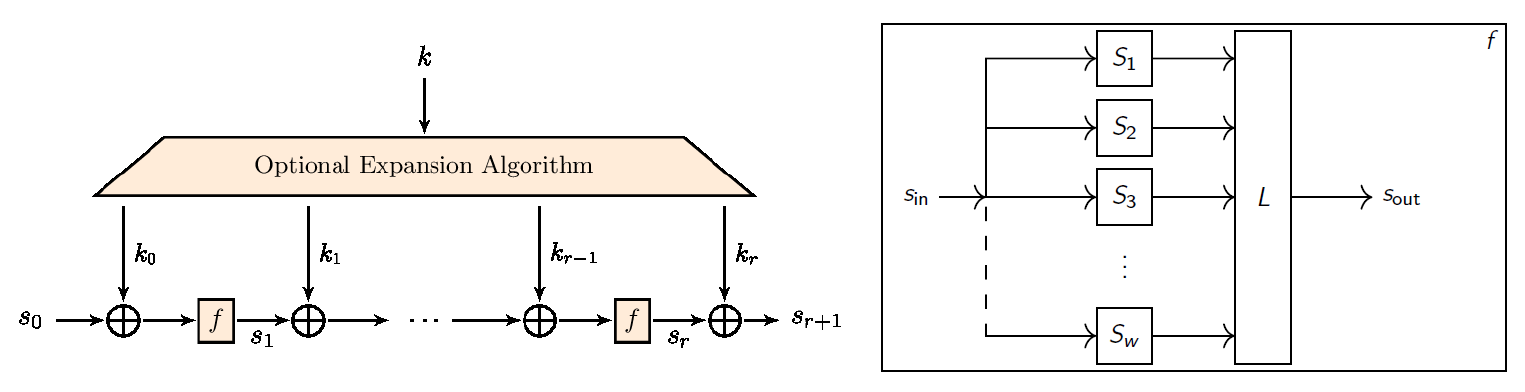
\includegraphics[width=162mm]{Graphics/Block Ciphers/bc1.png}
	\end{center}
	\begin{itemize}
	    \item Practical instantiation of the confusion-diffusion paradigm.
	    \item The S-boxes, key expansion algorithm and linear layer L are public.
	    \item The key is expanded to several subkeys that are mixed with the intermediate values using a bitwise XOR.
	    \item Subkeys are added before each round and after the last one.
	    \item The construction is invertible since both the S-boxes and the linear mixing layer are invertible.
	\end{itemize}


\section{The Avalanche Effect}
	\begin{itemize}
	    \item Example of design criterion to get the avalanche effect:
	    \begin{itemize}
	        \item the S-boxes are chosen so that changing a single bit of the input changes at least two bits of the output.
	        \item the mixing permutations (in that case simple bit reordering) are chosen so that the output bits of any given S-box are used as input of multiple S-boxes in the next round.
	    \end{itemize}
	    \item Consequence:
	    \begin{itemize}
	        \item a single bit difference between input blocks results in a difference of two bits after one round;
	        \item the second condition ensures that the inputs of at least two S-boxes of the second round will differ by one bit;
	        \item after the second round: at least 4 bits differ between the two blocks;
	        \item in the best case, $2^r$ bits will be affected after $r$ rounds (actually less);
	        \item this gives a lower bound for the number of rounds of an SPN: $$r \geq \lceil \log_2(n) \rceil$$
	    \end{itemize}
	\end{itemize}


\section{Feistel Networks}
	\begin{itemize}
	    \item Generic iterated structure to build a PRP from round functions.
	    \item Typically, round functions are also constructed from (possibly non-invertible) S-boxes and linear mixing layers.
	    \item Description of a round:
	    \begin{itemize}
	        \item break the block in two equal halves $L_i$ and $R_i$;
	        \item output $(L_{i+1},R_{i+1})$ defined as $L_{i+1} = R_i$ and $R_{i+1} = L_i \oplus f_i(R_i)$, where $f_i$ denotes 
	        the $i$-th (public) round function instantiated with a (secret) key $K$.
	    \end{itemize}
	    \item Inherently invertible: $R_i = L_{i+1}$ and $L_i = R_{i+1} \oplus f_i(L_{i+1})$.
	\end{itemize}
    \begin{center}
		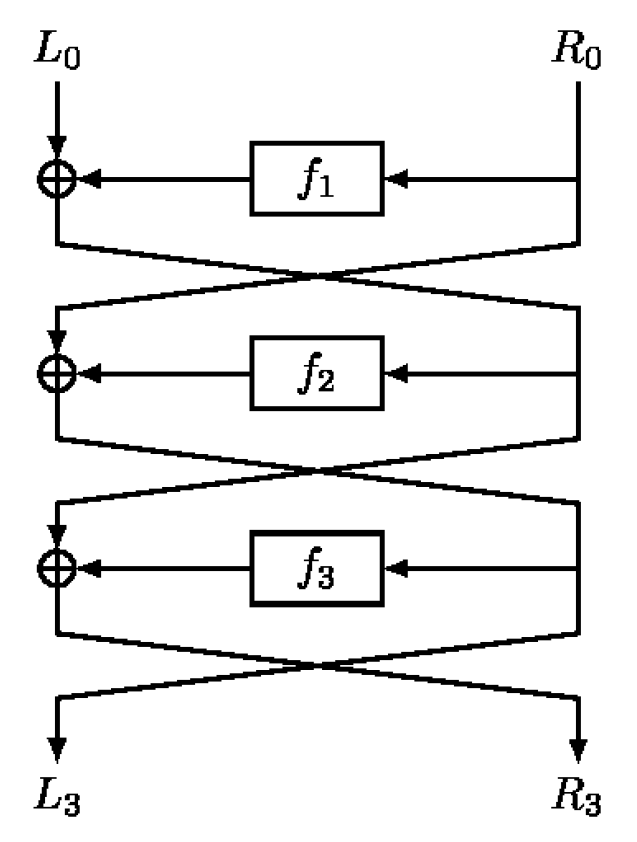
\includegraphics[width=68mm]{Graphics/Block Ciphers/bc2.png}
	\end{center}


\begin{theorem}[Feistel Networks]\ \\
	Assuming the round functions are uniformly random and independent
	functions from $\{0,1\}^n$ to $\{0,1\}^n$, then:
	\begin{itemize}
	    \item the $3$-round Feistel construction is $(q,\infty,\frac{q^2}{2^n})$-prp secure;
	    \item the $4$-round Feistel construction is $(q,\infty,\frac{q^2}{2^n})$-sprp secure;
	    \item the $6$-round Feistel construction is $(q,\infty,\frac{9q}{2^n})$-sprp secure secure as long as $q \leq 2^{n-7}$.\
	\end{itemize}

	\textbf{Interpretation of the theorem:}
	\begin{itemize}
	    \item actual block ciphers have simple round functions that are not random or pseudorandom;
	    \item however, the result justifies the soundness of the Feistel structure;
	    \item it provides lower bounds for the number of rounds that have to be used by an actual block cipher.
	\end{itemize}
	\end{theorem}


\section{Building Blocks of a Block Cipher}
	To summarize, the specification of a block cipher generally contains the following ingredients:
	\begin{itemize}
	    \item a high-level (iterated) structure (SPN, Feistel scheme,. . . );
	    \item a key-schedule algorithm to derive sub-keys from a master key;
	    \item small S-boxes that must be non-linear;
	    \item an efficient linear layer to properly spread local changes from the application of the S-boxes.
	\end{itemize}

\newpage
\section{Examples}
	\subsection{Example 1: The DES Block Cipher}
		\begin{itemize}
			\item DES was developed in the 1970s by IBM (+ some help from the NSA).
			\item Key length: 56 bits and block length: 64 bits.
			\item Although key length is too small for our current standards, it has been impressively resilient to decades of cryptanalysis.
			\item Best cryptanalysis: linear cryptanalysis using $2^{43}$ known plaintext/ciphertext pairs and time around $2^{40}$ DES evaluations.
		\end{itemize}
	    \begin{center}
			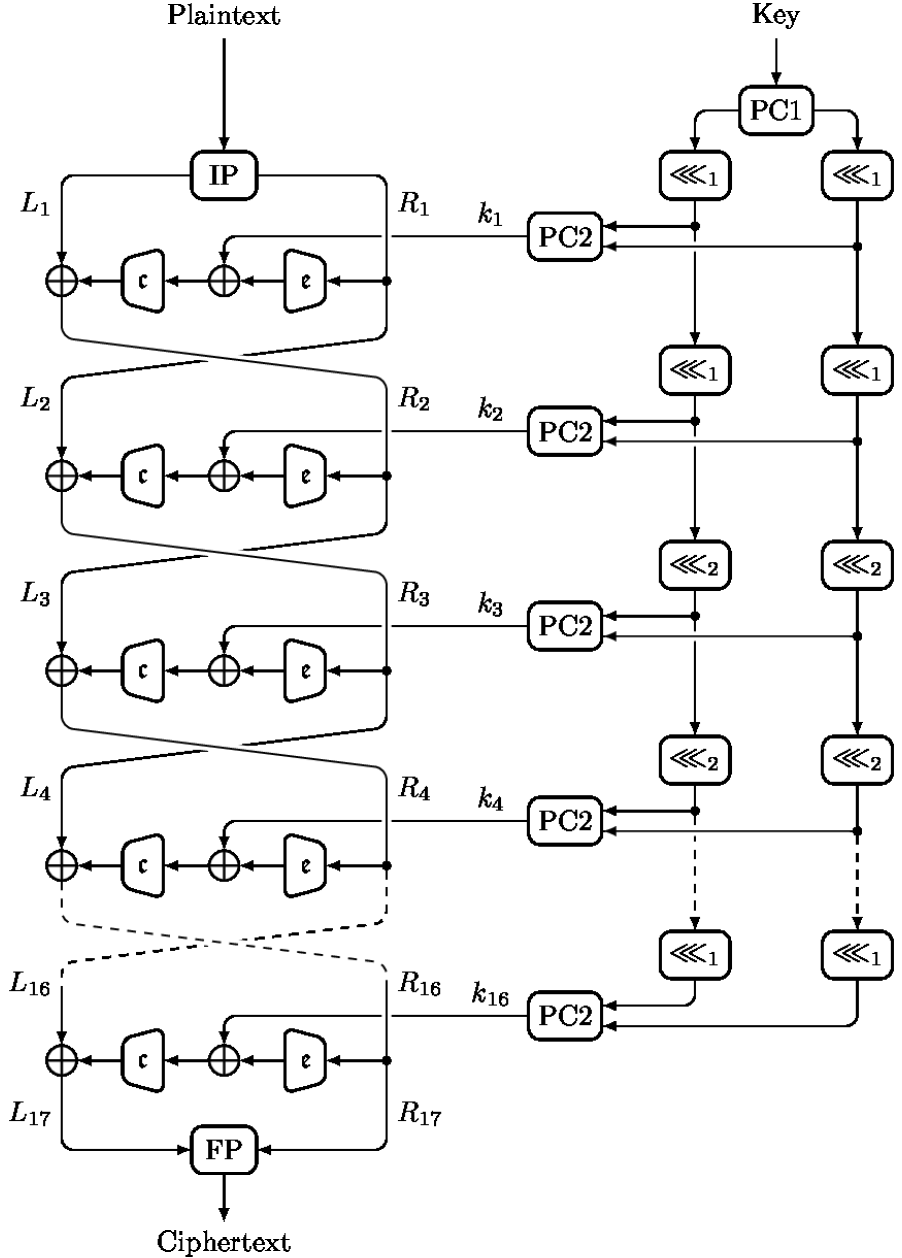
\includegraphics[width=88mm]{Graphics/Block Ciphers/bc3.png}
		\end{center}
		\begin{itemize}
			\item Generic structure: 16 round Feistel network.
			\item Key schedule:
			\begin{enumerate}
				\item PC1 splits the key in two 28-bit halves;
				\item both halves are rotated to the left before each round (number of places depends on the round);
				\item PC2 then extracts 48 key bits.
			\end{enumerate}
			\item IP and FP reorder the bits, but do not depend on any secret information (no impact on security).
			\item Round function:
			\begin{enumerate}
				\item e extends its 32-bit input to 48 bits;
				\item c contracts its 48-bit input back to 32 bits.
			\end{enumerate}
		\end{itemize}
	    \begin{center}
			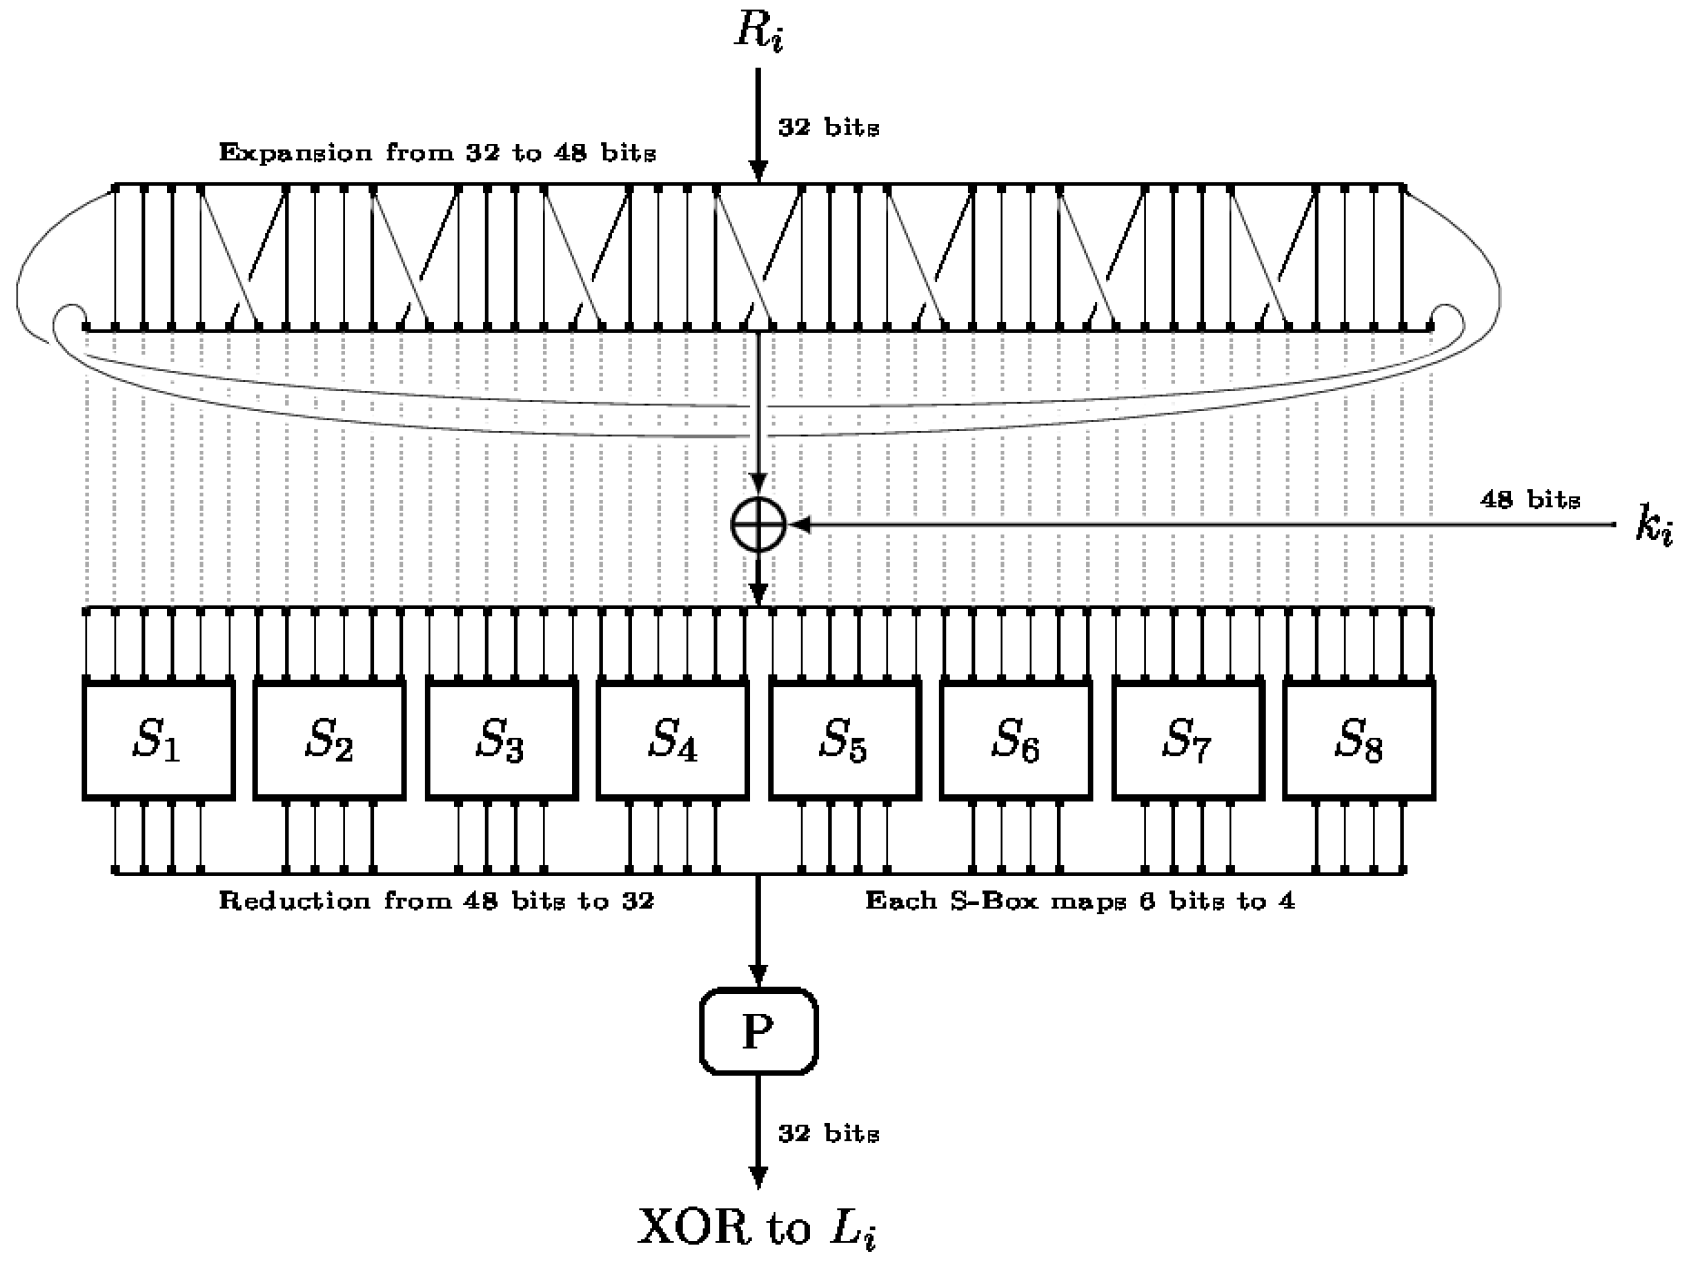
\includegraphics[width=160mm]{Graphics/Block Ciphers/bc4.png}
		\end{center}
		\begin{itemize}
			\item The S-boxes $S_1,...,S_8$ are 6-bit to 4-bit functions such that:
			\begin{enumerate}
				\item each S-box is 4-to-1;
				\item changing one bit of any input to an S-box always changes at least two bits of the output.
			\end{enumerate}
			\item the mixing layer $P$ is a simple reordering of the input bits such that the 4 output bits of any S-box 
			will affect the input to 6 S-boxes in the next round (thanks to the linear expansion layer e).\\
		\end{itemize}
		\textbf{The DES avalanche effect:}
		\begin{enumerate}
			\item Assume $(L_0,R_0)$ and $(L'_0,R'_0)$ are two inputs to the cipher such that $R_0 = R'_0$, $L_0$ and $L'_0$ differ by exactly one bit.
			\item After the first round, since $R_0 = R'_0$, then $L_1 = L'_1$, $R_1$ and $R'_1$ differ by exactly one bit.
			\item Since $L_1 = L'_1$, $R_2$ and $R'_2$ differ by at least 2 bits, while $L_2$ and $L'_2$ differ by exactly one bit.
			\item Thanks to $P$, the 2 different bits of $R_2$ and $R'_2$ appear in at least 2 S-boxes, which means that the new intermediate values will differ in at least 4 positions.
			This results in at least 2 different bits between $L_3$ and $L'_3$ and at least 4 different bits between $R_3$ and $R'_3$.
			\item We observe a similar exponential effect as in the Substitution-Permutation Network case.
		\end{enumerate}

\newpage
	\subsection{The AES Block Cipher}
		\begin{itemize}
			\item United States National Institute of Standards and Technology (NIST) standard adopted in 2000 after an open competition.
			\item Based on the winner of the competition: Rijndael (designed by Vincent Rijmen and Joan Daemen).
			\item Actually a set of 3 algorithms with block length 128 bits and key length 128, 192 or 256 bits.
			\item The length of the key affects the number of rounds (10, 12 or 14) and the key schedule.
			\item Modern processors support instruction sets to accelerate the computation of AES in hardware: around 4.5GB/sec for AES-128 in CTR mode 
			on an Intel(R) Core(TM) i7-3740QM CPU @ 2.70GHz (Fedora 31, openssl 1.1.1d)
			\item Best cryptanalysis: there exist attacks that recover the AES key with a computational complexity of $2^{126}$ operations for AES-128, 
			$2^{189}$ operations for AES-192, and $2^{254}$ operations for AES-256.
			No practical threat to the security of the cipher.
			\item Better attacks exist if the adversary is given more power (the ability to XOR any constant of its choice to the secret key), 
			but this does not impact the security of AES when used in standard modes of operation.
			\item Generic structure: 10, 12 or 14-round Substitution-Permutation Network.
			\item Key schedule: relies on linear operations and on the AES S-box, and outputs one 128-bit sub-key for each round, plus a final one.
			\item The AES round permutation consists in four steps:
			\begin{itemize}
				\item AddRoundKey: the bitwise XOR of the round key;
				\item SubBytes: the application of a single invertible S-box to each of the 16 bytes of the input;
				\item ShiftRows: a reordering of the bytes of the state;
				\item MixColumns: the application of a linear operation to the state.
			\end{itemize}
			\item In the last round, the MixColumns operation is skipped, and replaced with the XOR of the last key.
		\end{itemize}
	    \begin{center}
			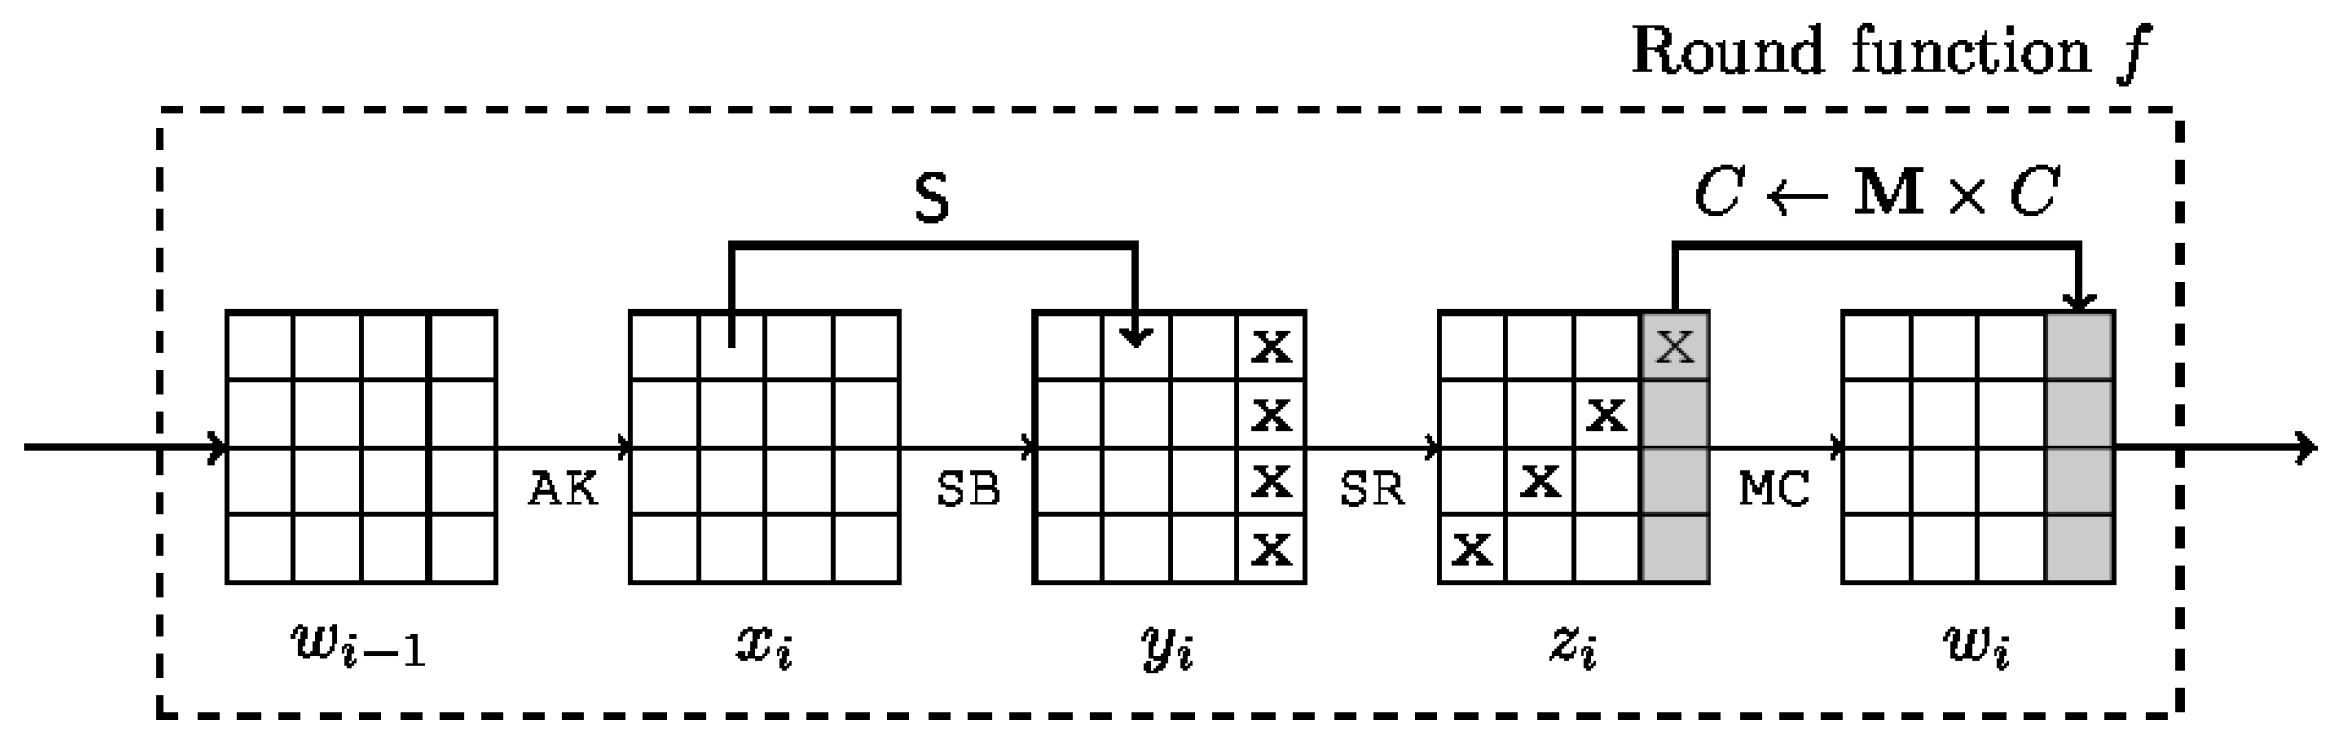
\includegraphics[width=140mm]{Graphics/Block Ciphers/bc5.png}
		\end{center}
		\begin{itemize}
			\item The block is seen as a $4 \times 4$ matrix of bytes.
			\item SubBytes applies the AES S-box to each element of the matrix.
			\item ShiftRows cyclically shifts row $r$ of the matrix by $r$ positions to the left for $r = 0,1,2,3$.
			\item MixColumns can be seen as the multiplication of each column of the matrix by a fixed invertible $4 \times 4$ matrix.
			This transformation has the property that, if two inputs differ in $b > 0$ bytes, then the outputs will differ in at least $5-b$ bytes.
		\end{itemize}
\newpage
		\textbf{The AES avalanche effect:}
		\begin{enumerate}
			\item Assume $X_0$ and $X'_0$ are two inputs to the cipher that differ in exactly one byte.
			\item After the first ShiftRows step, they will still differ in exactly one byte.
			However, at the end of the first round, all the bytes of the corresponding column will differ between both intermediate values, while the remaining bytes will stay equal.
			\item After the second ShiftRows step, there will be exactly one byte per column that will differ between both intermediate values.
			\item At the end of the second round, all bytes will be different between both intermediate values.
		\end{enumerate}

\section{Blockcipher Modes of Operation}
	\subsection{Using Block-Ciphers}
		\begin{itemize}
			\item Block ciphers/PRPs are a \textit{primitive}
			\item How do we construct encryption from PRPs?
			\item Constructions of encryption from block ciphers are called \textbf{modes of operation}
			\item Assume messages can be chopped into blocks of size $\lambda$, otherwise use padding
		\end{itemize}
	    \begin{center}
			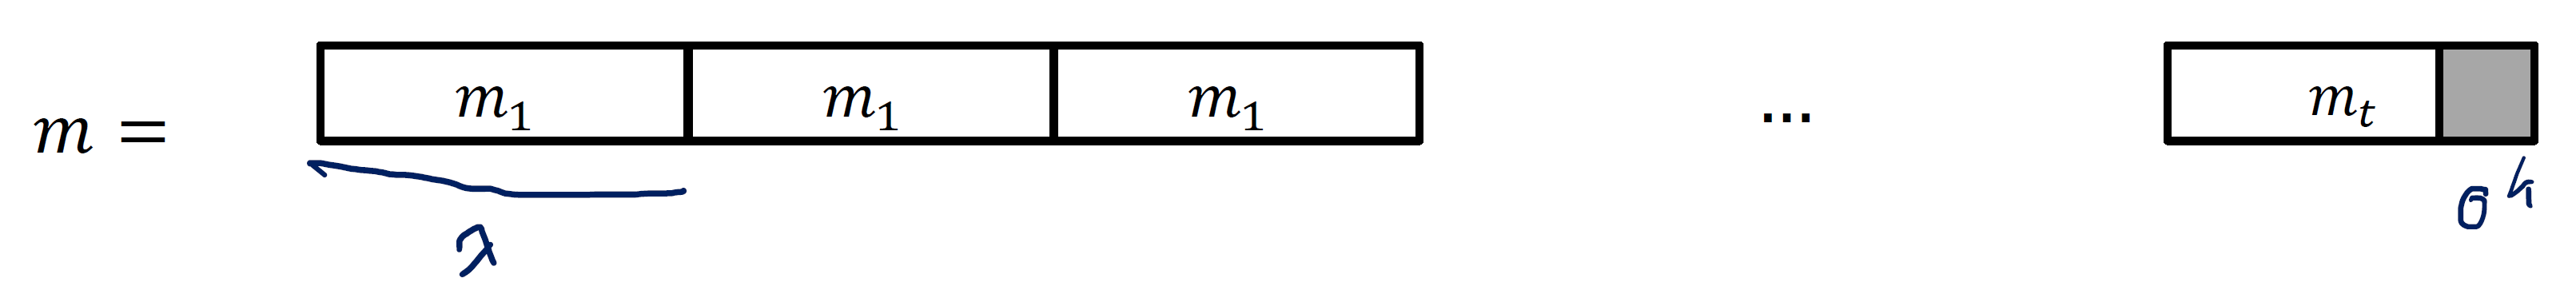
\includegraphics[width=160mm]{Graphics/Block Ciphers/bc6.png}
		\end{center}
	
	\subsection{Electronic Codebook Mode (ECM)}
		\begin{center}
			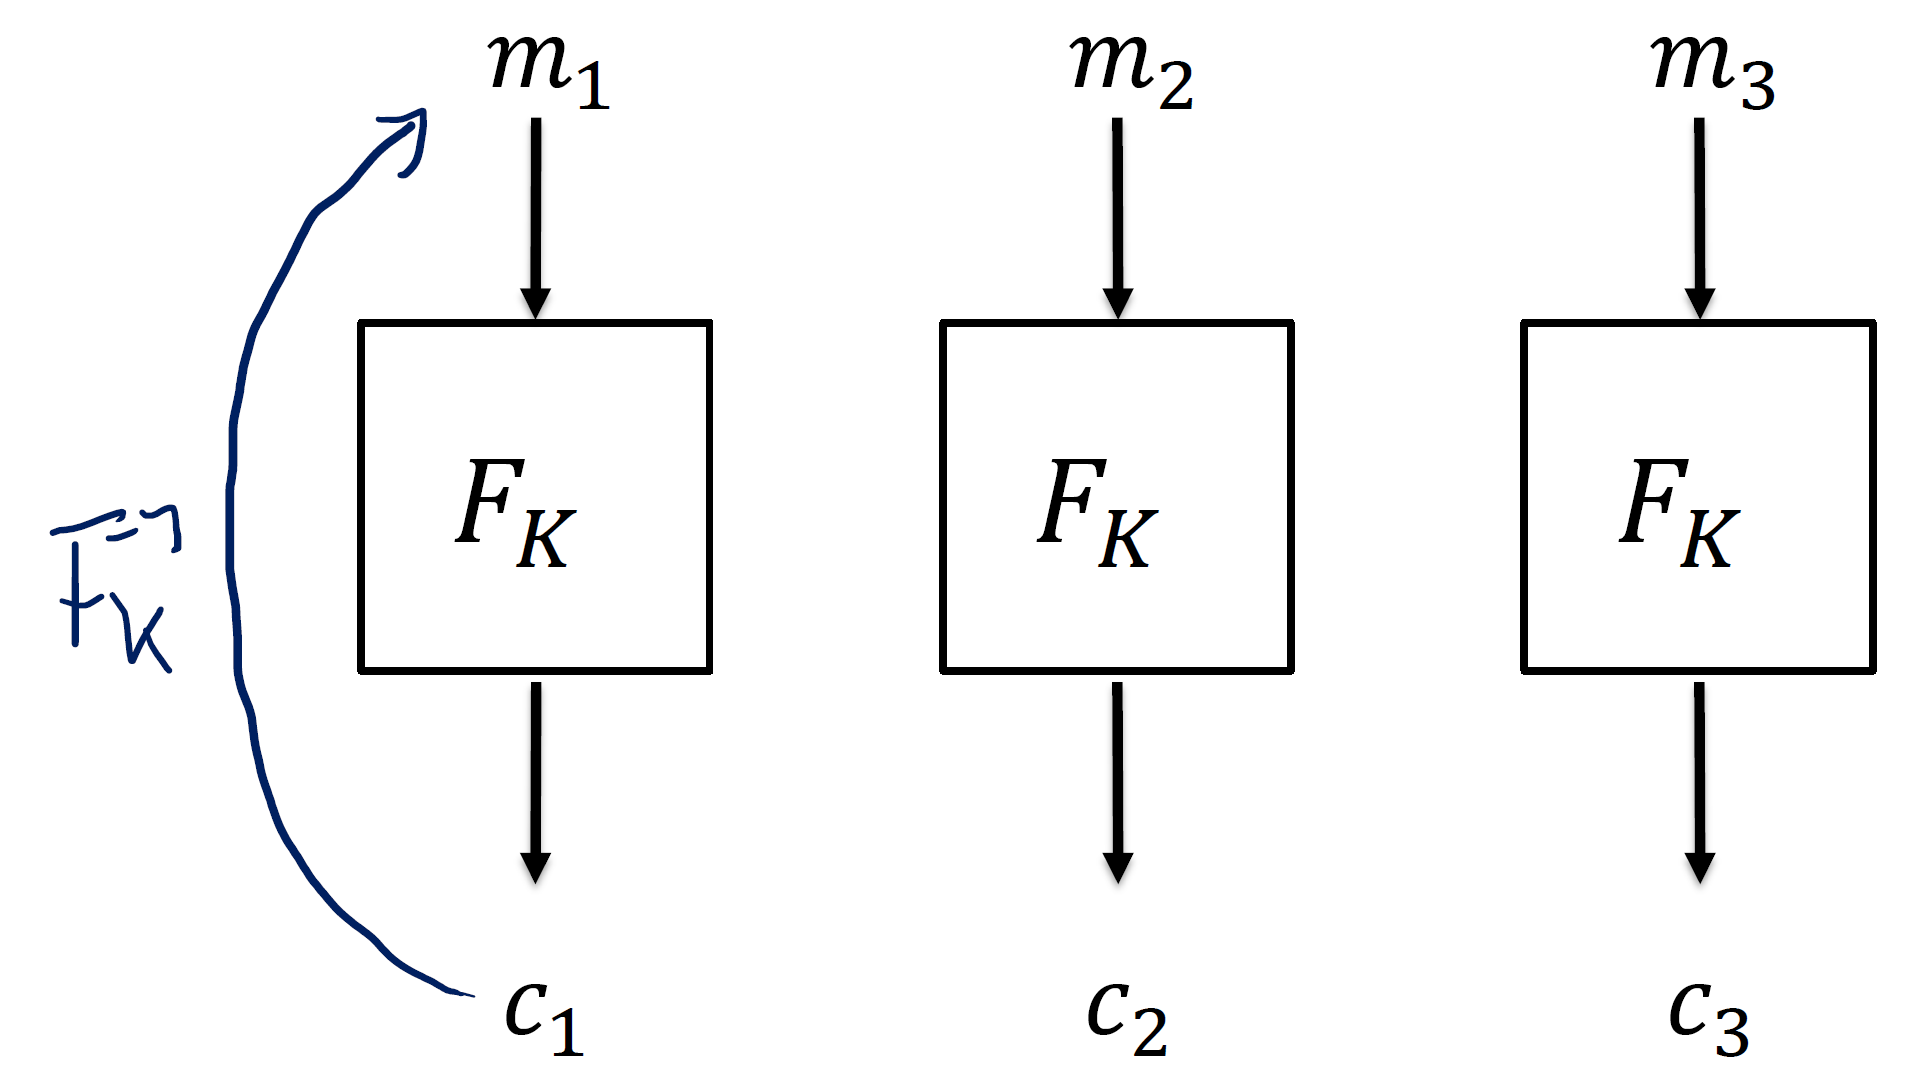
\includegraphics[width=140mm]{Graphics/Block Ciphers/bc7.png}
		\end{center}
		\begin{itemize}
			\item Not IND-CPA secure!
			\item Not even IND secure!
			\item Should not be used!
		\end{itemize}
		\begin{center}
			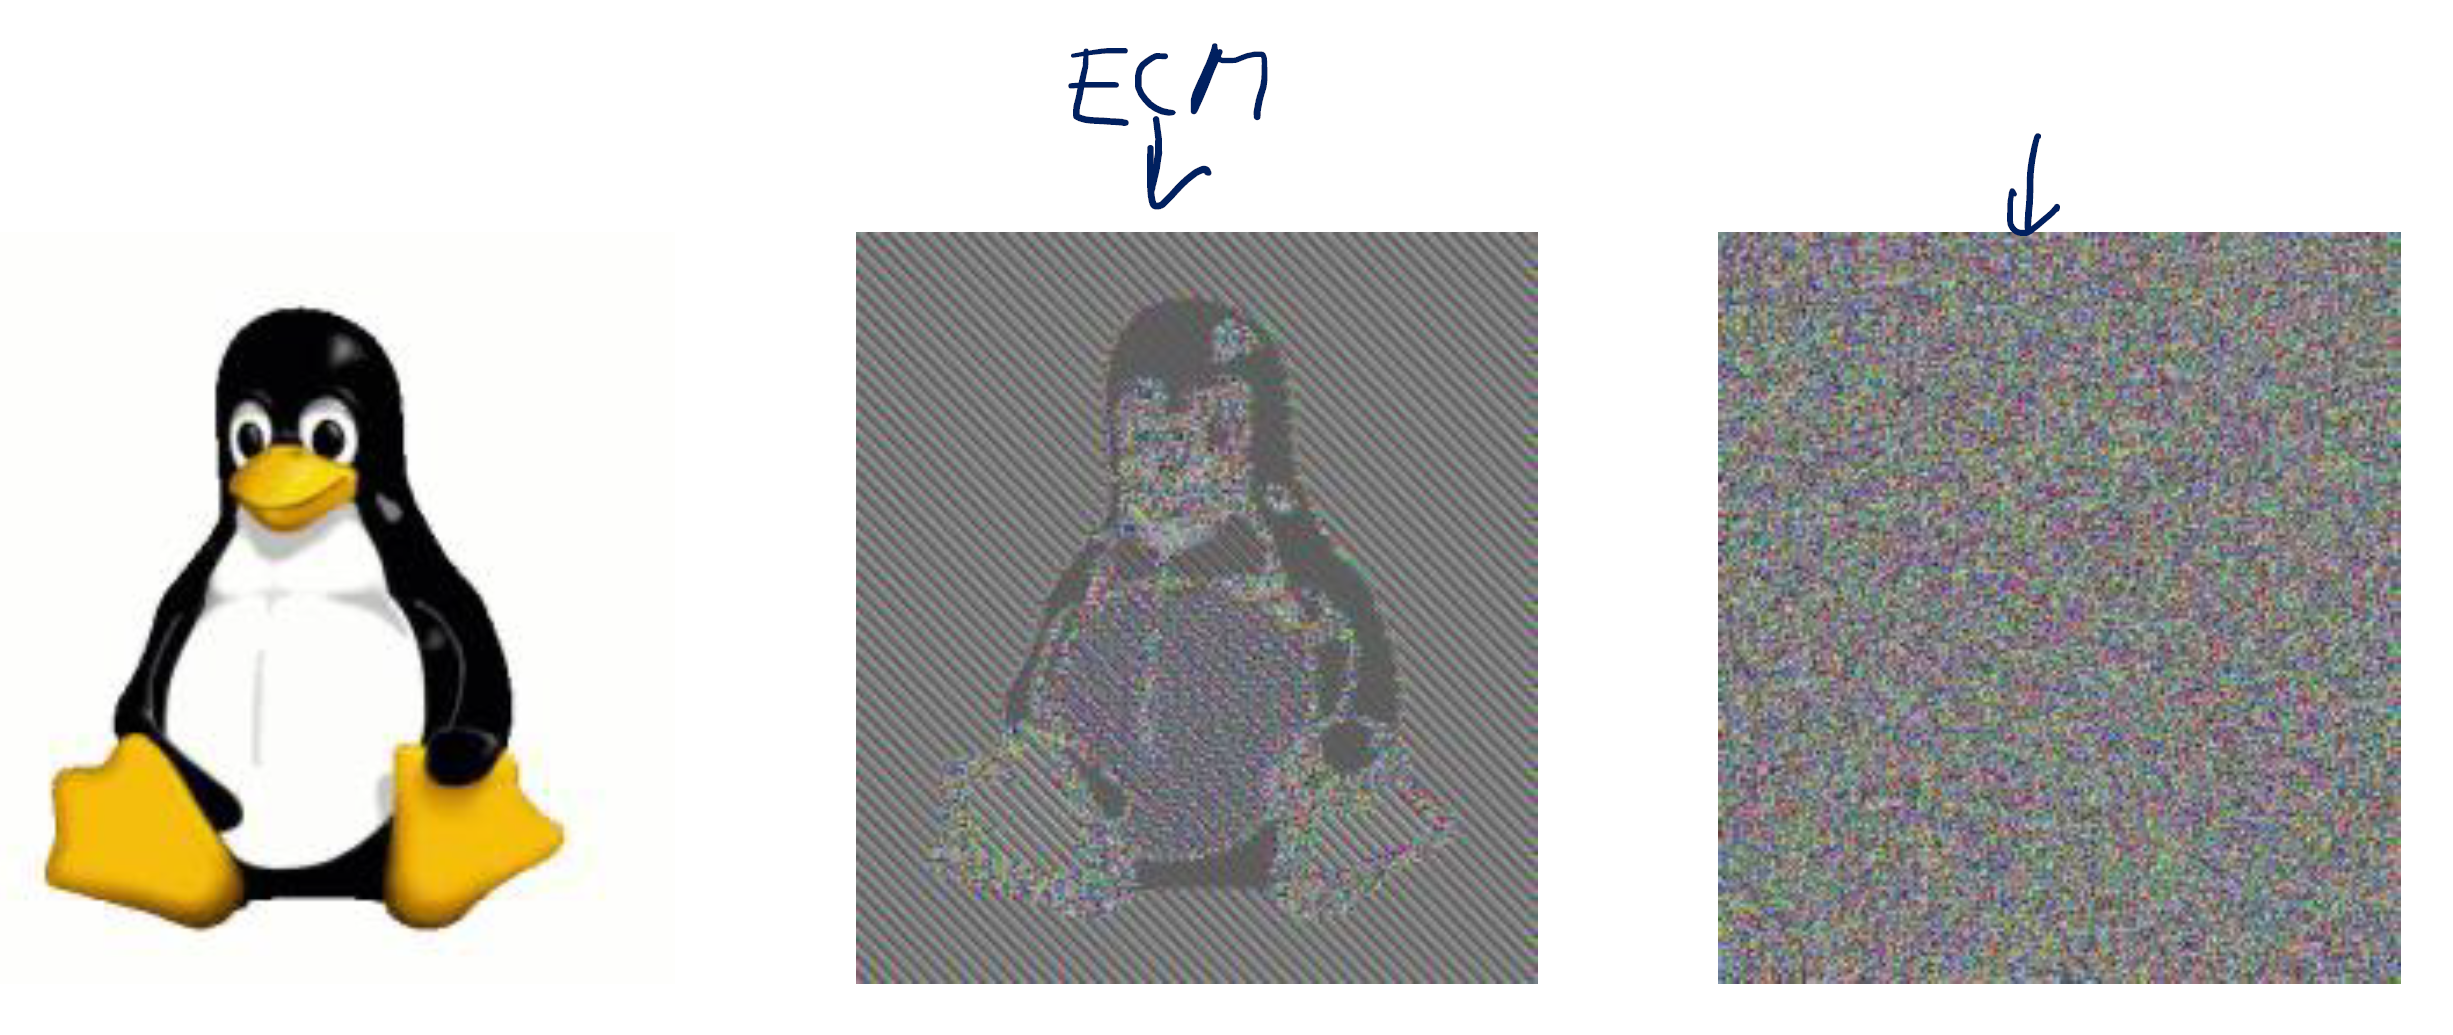
\includegraphics[width=160mm]{Graphics/Block Ciphers/bc8.png}
		\end{center}
	
	\subsection{Cipher Block Chaining (CBC) Mode}
		\begin{center}
			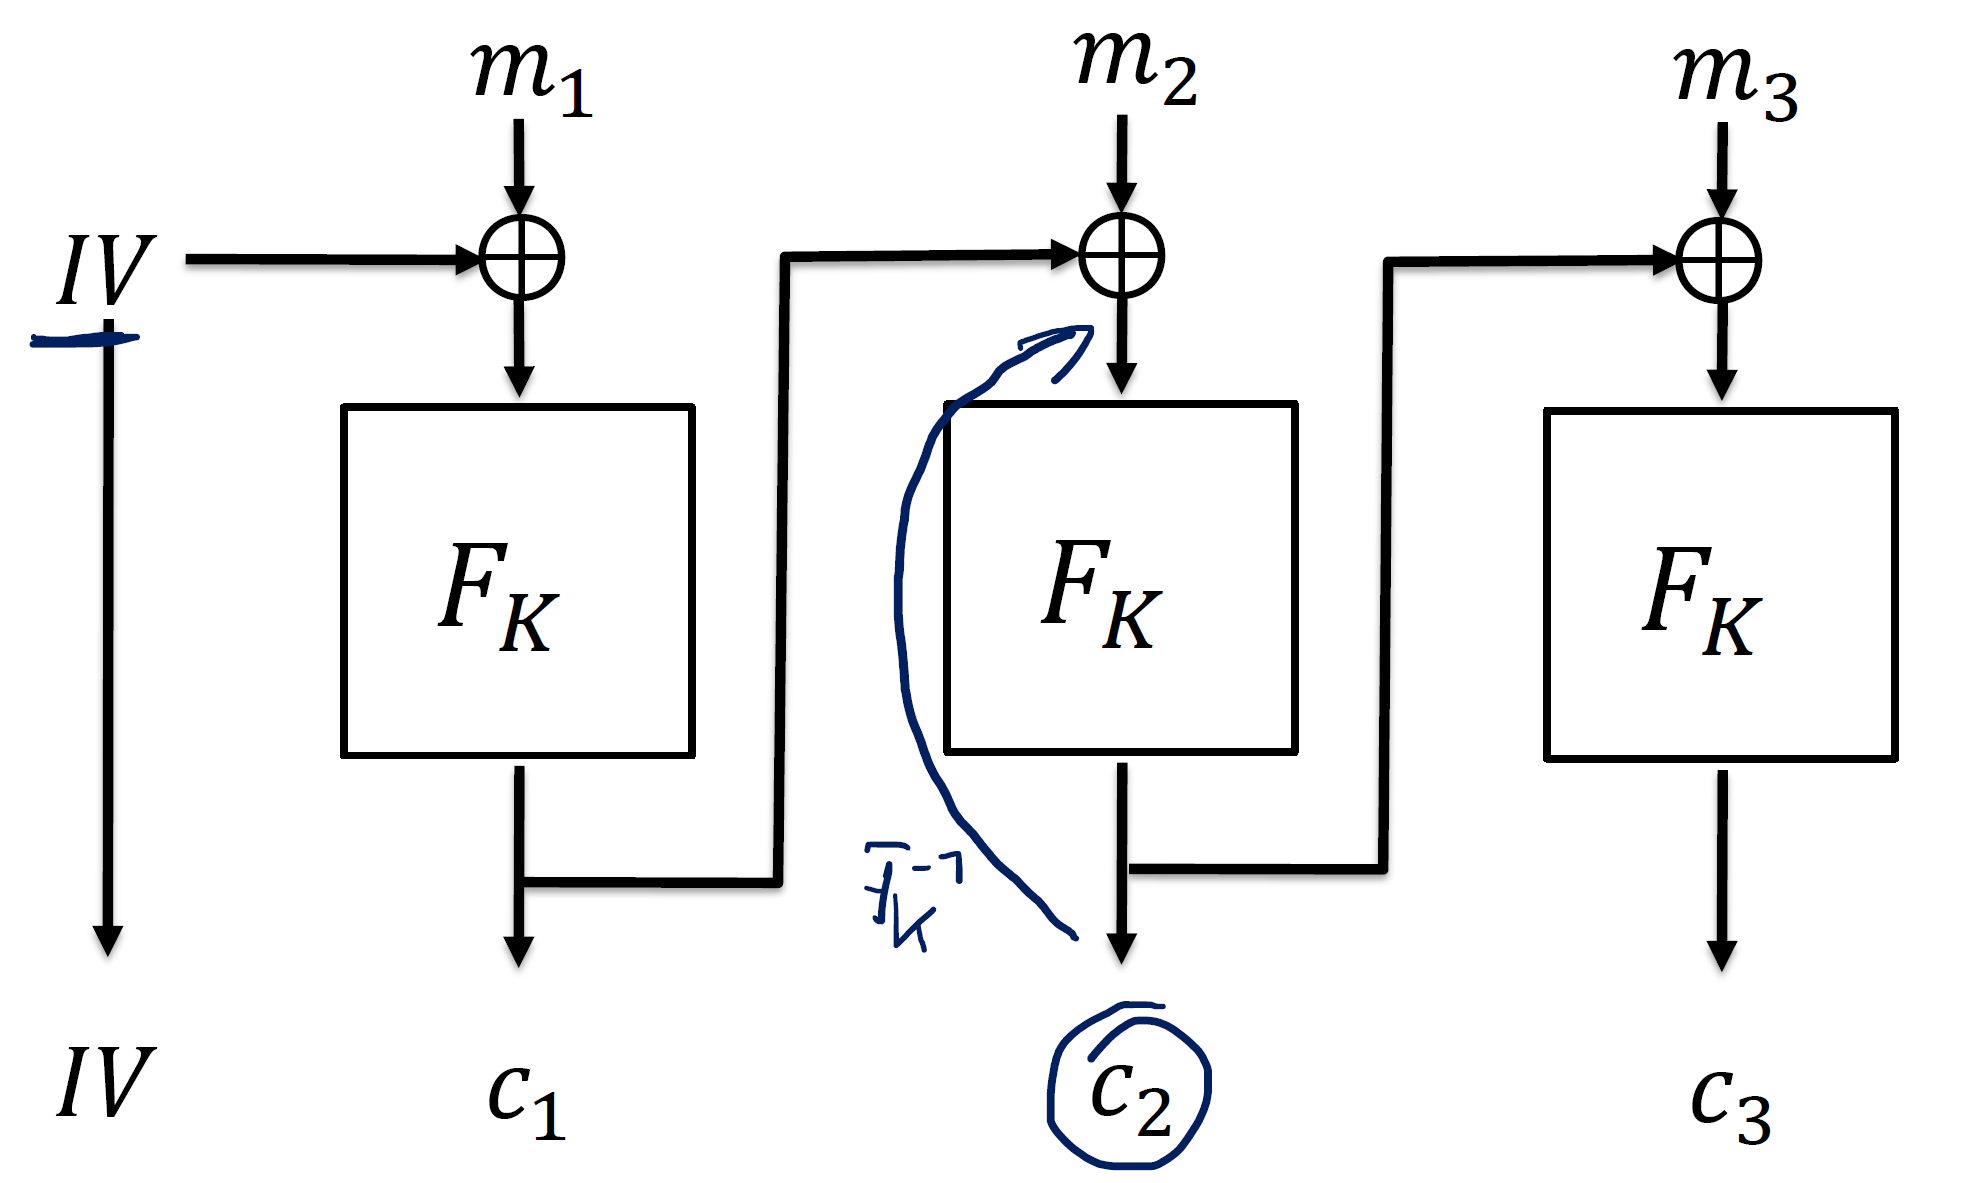
\includegraphics[width=120mm]{Graphics/Block Ciphers/bc9.png}
		\end{center}
		\begin{itemize}
			\item IND CPA secure for uniformly random IV if 𝐹is PRP
			\item Encryption must be performed sequentially
			\item Decryption is local
		\end{itemize}
	
	\subsection{Chained CBC Mode}
		\begin{center}
			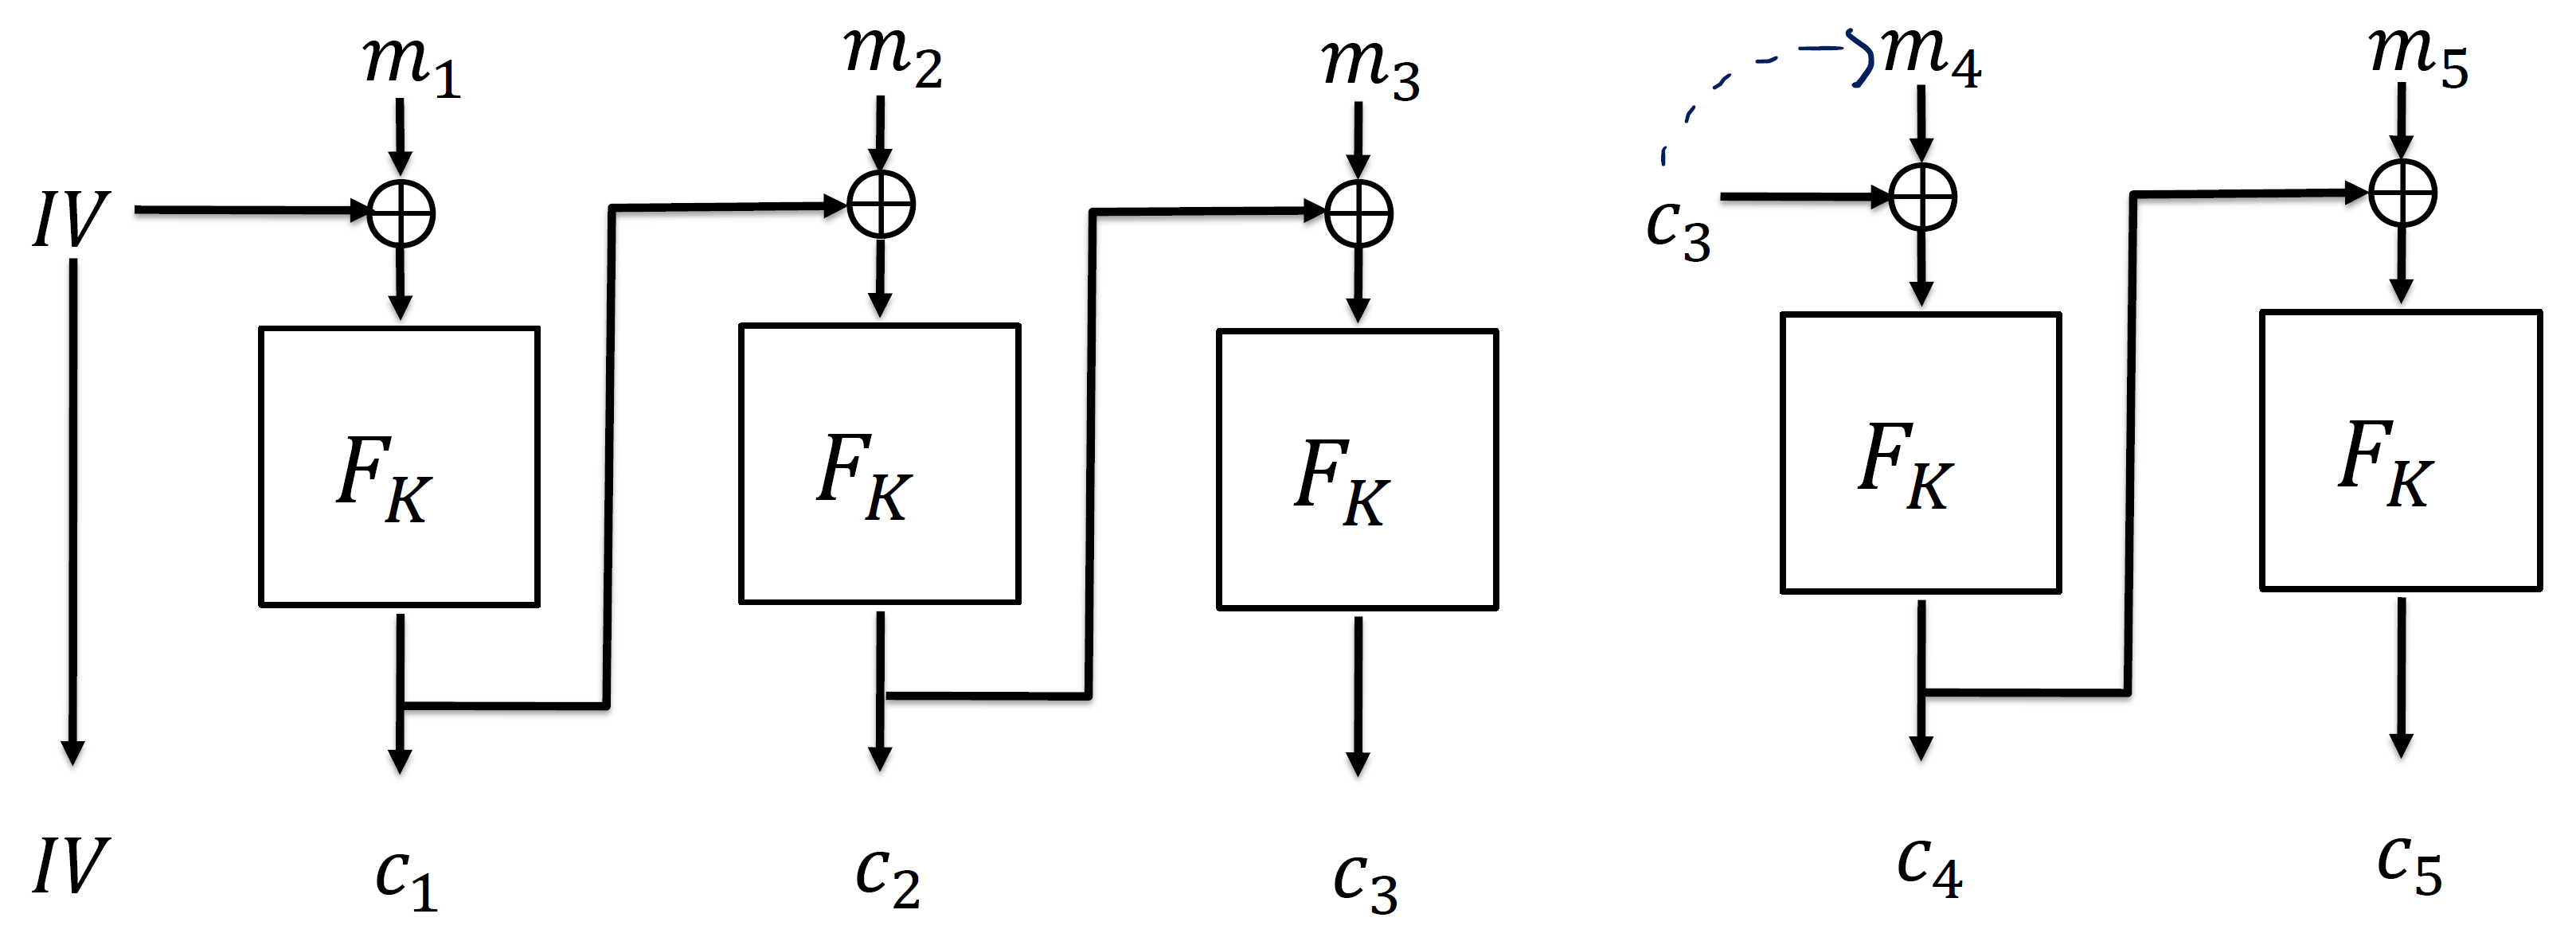
\includegraphics[width=120mm]{Graphics/Block Ciphers/bc10.png}
		\end{center}
		\begin{itemize}
			\item \textbf{Not} IND-CPA secure!
		\end{itemize}
	
	\subsection{Output Feedback (OFB) Mode}
		\begin{center}
			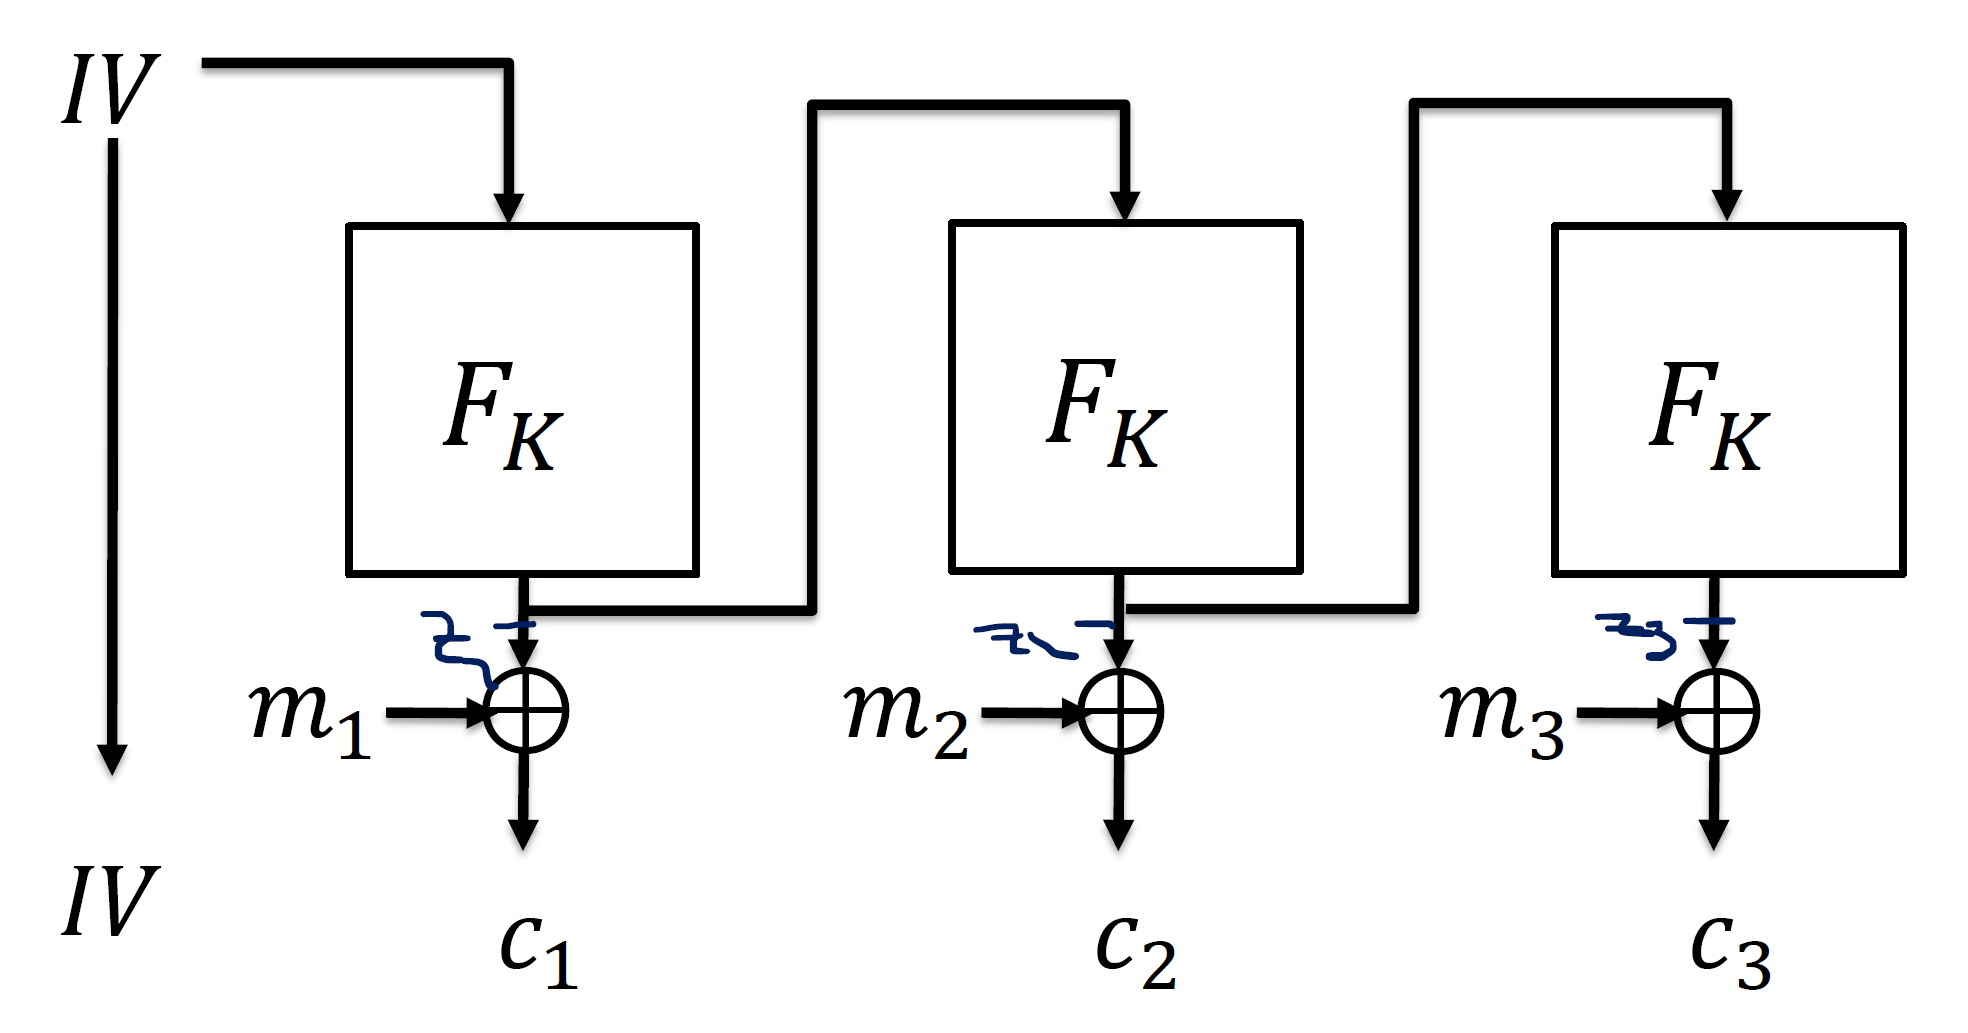
\includegraphics[width=120mm]{Graphics/Block Ciphers/bc11.png}
		\end{center}
		\begin{itemize}
			\item IND-CPA secure for uniformly random IV if $F$ is PRF
			\item Encryption and Decryption must be performed sequentially!
			\item Pad can be precomputed
		\end{itemize}
	
	\subsection{Counter (CTR) Mode}
		\begin{center}
			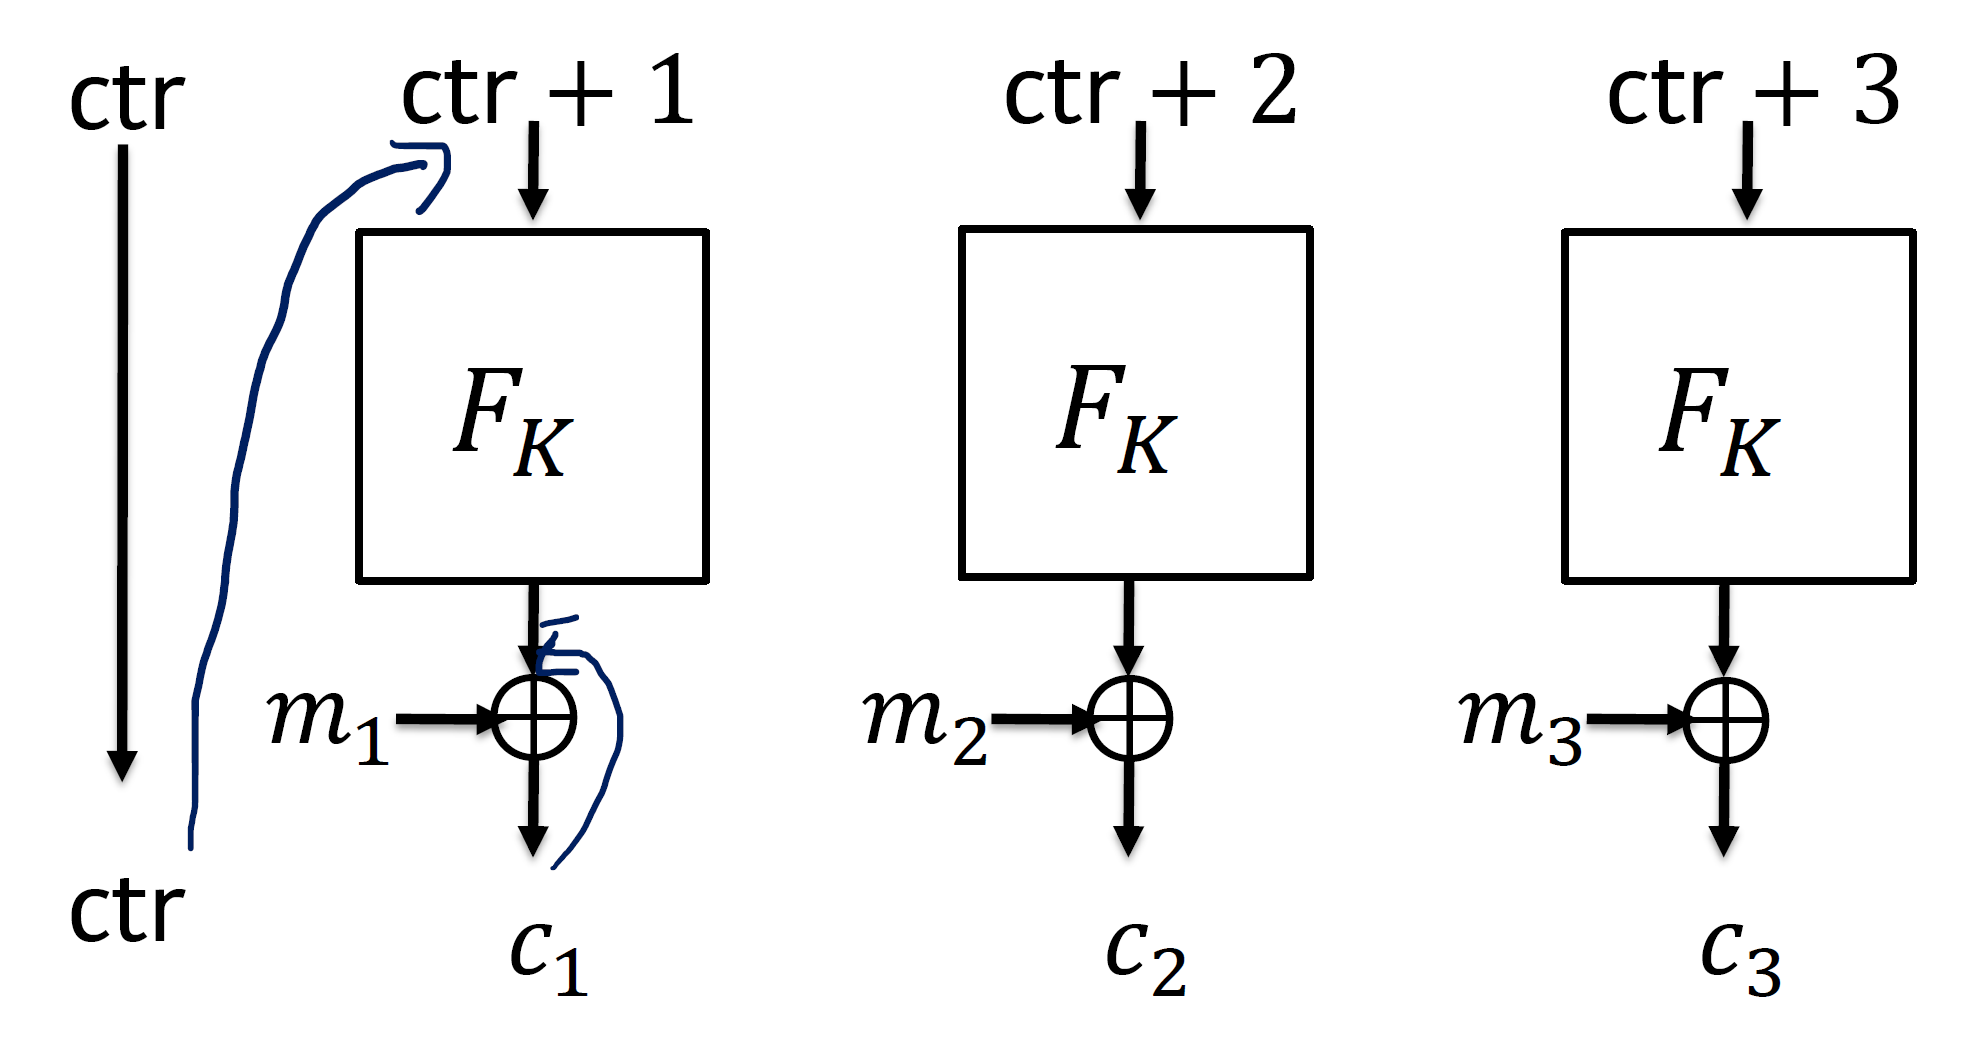
\includegraphics[width=120mm]{Graphics/Block Ciphers/bc12.png}
		\end{center}
		\begin{itemize}
			\item IND-CPA secure for uniformly random ctr if $F$ is PRF
			\item Encryption and Decryption are local/can be parallelized/precomputed
			\item Not reason not to use this one!
		\end{itemize}

\section{Summary}
	\begin{itemize}
		\item Blockcipher modes of operation provide a way to encrypt long messages
		\item ECM provides very little security $\rightarrow$ should only be used in very special scenarios
		\item CBC is ok!
		\item Chained CBC is not ok!
		\item OFM is ok!
		\item Use CTR whenever possible!
	\end{itemize}























